% kate: default-dictionary nl;

\documentclass[a4paper,12pt]{article}

\usepackage[ansinew]{inputenc}


\newcommand{\subTitle}{Robots and Society: report 3}
\newcommand{\authorName}{Moens Karel}
\newcommand{\authorCode}{33Z12022}

\title{Project MCS: Logical Pacman \\ Iteraties 2 \& 3}
\author{Jessa Bekker\\s0215494 \and Karel Moens \\ s0215430 }
\date{\today}

\setlength{\parskip}{\baselineskip}%
\setlength{\parindent}{0pt}%
	
\usepackage[dutch]{babel}
\usepackage{graphicx, flafter}
\usepackage{amssymb, amsmath}
\usepackage{pdfpages}
\usepackage{subfigure}
\usepackage{placeins}
\usepackage{hyperref}
\usepackage[backend=bibtex]{biblatex}

\begin{document}
\maketitle

% control+d		: comment
% control+shift+d	: uncomment

\section{Inleiding}
In dit verslag worden kort de ontwerpbeslissingen bij het uitwerken van het tweede en derde deel van het project toegelicht.
De opdracht van het tweede deel was de modellering van het pacman spel  in IDP met behulp van het LTC-formalisme en het uitvoeren van enkele verificaties daarop om de correctheid van de oplossing te testen.
De opdracht van het derde deel was de modellering van het pacman spel in NuSMV en daar een aantal invarianten te bewijzen met behulp van LTL en CTL.
Tot slot vermeldt de tekst ook de tijd die nodig was om dit te verwezenlijken.

\section{IDP}
\subsection{Toestandsaxioma's}
De meeste toestandsaxioma's konden overgenomen worden uit de oplossing voor iteratie 1 door een tijd variable toe te voegen. \texttt{PreviousMove} werd ook behouden (met tijdsvariabele), dit predicaat laat toe binnen \'e\'en toestand te redeneren. Enkele verbeteringen op vlak van complexiteit en performantie waren mogelijk. Voor de performantie werd de voorwaarde dat alle vakjes elkaar moeten bereiken versoepeld naar dat \'e\'en vakje alle andere moet kunnen bereiken, wat hetzelfde impliceert. Verder werd het predicaat \texttt{Edge(x1,y1,x2,y2,d)} toegevoegd dat verschillende voordelen geeft. Edge drukt de relatie uit tussen 2 aangrenzende vakjes op posities (x1,y1) en (x2,y2) waarvan vakje 2 in richting d ten opzichte van vakje 1 ligt. Als vakjes een gemeenschappelijke \texttt{Edge} hebben, betekent het dat er geen muur tussen staat en dat ze beide posities zijn. Dit wordt gebruikt om \texttt{Reach(x1,y1,x2,y2)} effici\"enter na te gaan door enkel naar buren te kijken en niet naar eender welk vakje. Het 
wordt ook gebruikt om mogelijke stappen te vinden (die niet door een muur, van het bord af of naar een NoPos gaan), wat gebruikt wordt als voorwaarde op \texttt{Move} en de 2 nieuwe toestandsaxioma's: \texttt{DeadEnd} en \texttt{Crossed}. De implementatie wordt hierdoor minder complex.

\subsection{Fluents}
\texttt{GameWon} en \texttt{GameLost} zijn net zoals \texttt{Position} en \texttt{Gold} fluents. Inertie is duidelijk van toepassing op hun omdat hun waarde hetzelfde blijft tenzij die verandert door de toestand van het spel. \texttt{GameWon} en \texttt{GameLost} hebben onmiddelijke causaties. Dit komt doordat ze afhankelijk zijn van de toestand. Als er een winnende toestand is, dan is het spel dan gewonnen en niet pas in de volgende toestand.

\subsection{Verificatie}
De eerste twee verificaties zijn voorwaarden waar altijd, in alle mogelijke modellen, aan voldaan moet zijn. De manier om dit na te gaan is contradictie: de omgekeerde voorwaarde toevoegen. Als de theorie met deze bijkomende voorwaarde satisfieerbaar is, betekend dat dat aan de originele voorwaarde niet voldaan werd. Als er zo geen modellen bestaan dan is het wel correct.

De laatste twee verificaties stellen dat er een model moet bestaan waarin aan een voorwaarde voldaan is. Om dit te controleren wordt de voorwaarde toegevoegd en nagegaan of er een model voor bestaat. Het verschil tussen de eerste twee verificaties en de laatste twee is dat het bij de eerste in alle modellen voldaan moet zijn en in de laatste in minimum 1 model.

De eerste verificatie (het aantal muntstukken op het bord kan enkel omlaag gaan) gebeurt door de voorwaarde toe te voegen dat er op een tijdstip geen goud ligt op een vakje maar op een later tijdstip, op dat zelfde vakje, plots wel. Dit werd verkozen boven de letterlijke vertaling van de opgave omdat het strikter (muntstukken kunnen ook niet van vakje veranderen) en performanter is. Deze striktere voorwaarde impliceert wel dat het aantal muntstukken op het bord enkel omlaag kan gaan.

In alle gegeven en enkele zelf geschreven test-structuren wordt er aan de verificaties gedaan met uitzondering van de volgende gevallen:
\begin{itemize}
\item Er bestaan modellen voor de test-structuren, anders kan er nooit gewonnen of verloren worden.
\item In een test-structuur waar elk altijd gewonnen of verloren wordt, faalt de verificatie dat het spel altijd verloren, respectievelijk gewonnen, moet kunnen worden.
\end{itemize}


\section{NuSMV}

\subsection{Modellering}

\subsubsection{Direction en bewegen}
Pacman en ghost bevinden zich in een co\"ordinaten systeem.
Bij elke stap verandert of $ x $ of $ y $ met $ 1 $
maar ter beperking van het aantal mogelijke toestanden, is $ 4 $ de maximale waarde voor beide.
Dit zou zonder problemen naar een willekeurig getal groter dan $ 4 $ verhoogd kunnen worden.

Om te voorkomen dat ghost rechtsomkeer maakt, 
en om muren ondoordringbaar te maken,
werd aan \texttt{agent} instanties een variabele \texttt{direction} toegevoegd.
In combinatie met de huidige co\"ordinaten bepaalt deze volledig en deterministisch de volgende positie van de \texttt{agent}.
Daarom kan de volgende \texttt{direction} van een \texttt{agent} die ghost is,
niet het tegengestelde van de huidige richting zijn, vandaar de parameter \texttt{isGhost}.

Op een gelijkaardige manier werden in de module \texttt{square} invarianten toegevoegd
die de volgende richting beperken tot deze waarin geen muren staan
wanneer respectievelijk pacman of ghost zich op dat vakje bevinden.
Ook dit verklaart waarom een \texttt{square} bij creatie verwijzingen krijgt naar pacman en ghost.

\subsubsection{Coins}
De variabele \texttt{contains\_coin} bepaalt of er op een \texttt{square} nog goud ligt.
Bij het begin van het spel ligt overal behalve waar pacman start goud.
In elke volgende toestand verdwijnt het goud op een vakje als pacman tijdens die beurt daar zal staan.
Daarnaast verandert de variabele \texttt{contains\_coin} niet.

\subsubsection{GameState}
\texttt{gameState} Kan drie waarden aannemen: $ playing $, $ WIN $, $ LOSE $.
Vanaf de start is \texttt{gameState} $ playing $.
In de toestanden die daarop volgen wordt telkens eerst gecontroleerd of de speler zal verliezen.
Zo niet, kijkt de implementatie of alle goudstukken zullen verdwenen zijn en hij zal winnen.
Wanneer ook dit niet het geval is, blijft de huidige \texttt{gameState} behouden.

De speler verliest niet alleen wanneer pacman een vakje deelt met ghost,
maar ook als pacman en ghost elkaar kruisen.
Zo is het spel in de volgende toestand verloren wanneer pacman en ghost naast elkaar staan,
enkel hun $ x $ of $ y $ co\"ordinaat verschilt met $ 1 $, en ze van plan zijn naar elkaar te bewegen.

\subsection{Verificatie}
De eerste verificatie vraagt dat het spel vanuit elke begintoestand gewonnen of verloren kan worden.
Omdat niet volledig duidelijk is wat de mogelijke begintoestanden zijn,
worden deze ge\"interpreteerd als alle toestanden.
Er bestaat altijd een toekomstige toestand waarin de speler verliest.
Bij het winnen moet de extra voorwaarde opgelegd worden dat hij niet in de volgende beurt verliest.
Het is namelijk zo dat de keuze van \texttt{direction} al deterministisch bepaalt of dat zal gebeuren.

Wanneer op het eerste vakje geen muntje ligt, zal er daar in alle volgende toestanden daar geen munt liggen.
Omdat vakjes steeds zeer algemeen beschreven werden, is dit voldoende om hetzelfde voor alle vakjes te garanderen.

% Om oneindig vaak op hetzelfde vakje te komen,
% moet er een uitvoering van het spel zijn waarin er voor elke toestand nog een latere toestand volgt 
% zodat pacman opnieuw dat vakje bereikt.

Na gaan dat er een uitvoering bestaat waarin pacman oneindig vaak op een specifiek vakje komt,
is een moeilijke kwestie.
Het is niet altijd zo dat hij meerdere keren op dat vakje komt dus zijn $ LTL $ formules niet bruikbaar.
Daarnaast bezit $ CTL $ niet de expressiviteit om uitspraken te doen over toekomstige toestanden 
binnen een zelfde uitvoeringspad.

Bekijk ter illustratie figuur \ref{fig:loops}. 
Stel dat dit een deel vormt van een groter transitiesysteem,
en dat men wil verifi\"eren dat er een pad bestaat waarin $ \neg p $ oneindig vaak voorkomt.
Het lijkt aannemelijk dat dit in $ CTL $ wordt $ EG\;EF\; \neg p $,
maar neem nu het pad die eeuwig in de eerste lus blijft hangen.
In elke toestand bestaat er een pad waarin $ p $ ooit vals wordt.
Dit gebeurt echter nooit in het gevonden pad.

Zo kan er in het pacman spel ook niet gegarandeerd worden dat de specifieke positie 
binnen een zelfde pad steeds bereikt wordt.
Het is wel mogelijk, en dit wordt ook in de implementatie gedaan,
om op te leggen dat pacman steeds naar dat vakje kan gaan.

Om uitspraken te doen over een bepaald uitvoeringspad is een $ CTL^{*} $ formule nodig, namelijk
\newline
$ E \; (\,G\;gameState = playing\; ->\; GF (\,pacman.x = 1\;\&\; pacman.y = 1\,)\,) $

\begin{figure}[h!]
\begin{center}
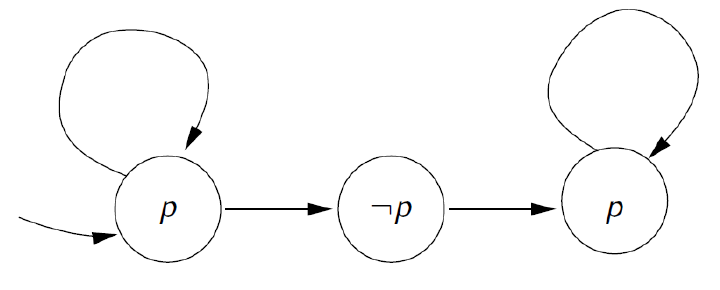
\includegraphics[width=0.6\columnwidth]{loops.png}
\end{center}
\caption{Een onderdeel van een algemeen transitiesysteem. 
De formule $ EG\;EF\; \neg p $ slaagt door de eerste lus.}%
\label{fig:loops}%
\end{figure}

Met $ LTL $ kan men wel nagaan dat als pacman oneindig vaak op twee specifieke vakjes komt,
hij nooit zal winnen.

Tot slot zijn er minstens $ 10 $ tijdstappen nodig als het spel in elke $ 9^{de} $ toestand nog niet gewonnen is.

\section{Tijdsbesteding}
\begin{tabular}{l l l}
Jessa: 	& IDP 	& $ 10\,u $\\
		& NuSMV 	& $ 4,5\,u $\\
Karel: 	& IDP 	& $ 4\,u $\\
		& NuSMV 	& $ 9\,u $\\
\end{tabular}

%\section{Besluit}

\end{document}